\documentclass[tikz,border=5pt]{standalone}
\usetikzlibrary{calc}
\begin{document}
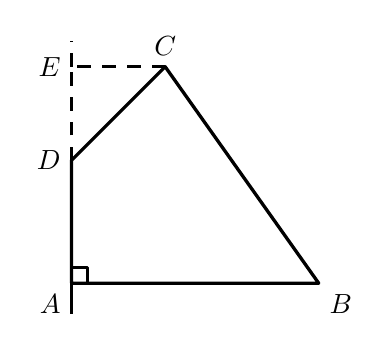
\begin{tikzpicture}[line width=1.2pt, line join=round]
% Named coordinates: 1 unit = 100 px, y flipped as (410 - y_px)/100
\coordinate (A) at (0.70,0.69);
\coordinate (B) at (3.84,0.69);
\coordinate (C) at (1.89,3.44);
\coordinate (D) at (0.70,2.25);
\coordinate (E) at (0.70,3.44);
\coordinate (S) at (0.70,0.30);   % solid stub end below A (y_px = 380)
\coordinate (T) at (0.70,3.76);   % dashed extension top (y_px = 34)

% Solid outline: A-B, B-C, C-D, D-A
\draw (A) -- (B) -- (C) -- (D) -- (A);
% Solid stub below A
\draw (A) -- (S);

% Dashed segments: D-E, E-C, and extension above E
\draw[dash pattern=on 5pt off 4pt] (D) -- (E) -- (C);
\draw[dash pattern=on 5pt off 4pt] (E) -- (T);

% Right-angle square mark at A (side 0.2 units = 20 px)
\draw ($(A)+(0.2,0)$) -- ($(A)+(0.2,0.2)$) -- ($(A)+(0,0.2)$);

% Point labels
\node[below left]  at (A) {$A$};
\node[below right] at (B) {$B$};
\node[above]       at (C) {$C$};
\node[left]        at (D) {$D$};
\node[left]        at (E) {$E$};
\end{tikzpicture}
\end{document}